% !TeX program = xelatex
\documentclass[a4paper,10pt]{article}

% ============================================================================
% កញ្ចប់បណ្ណាល័យ (Packages) – តាមលំនាំស្តង់ដារអនុវិទ្យាល័យព្រះក្រសាំង (ls_plan.tex)
% ============================================================================
\usepackage[a4paper, left=0.95cm, right=0.95cm, top=0.85cm, bottom=0.92cm, footskip=0.52cm]{geometry}
\usepackage{amsmath}
\usepackage{unicode-math}
\usepackage{fontspec}
\usepackage{array, longtable, multirow, colortbl}
\usepackage[table]{xcolor}
\usepackage{enumitem}
\usepackage{pifont}
\usepackage{fancyhdr}
\usepackage{tikz}
\usetikzlibrary{calc, arrows.meta, angles, quotes, decorations.markings, babel}

% LaTeX 2025 + longtable compatibility guard
\makeatletter
\let\@expl@@@mark@update@singlecol@structures@@\relax
\makeatother

% ============================================================================
% ការកំណត់ពុម្ពអក្សរ (Cross-Platform Windows + Linux Cloud fonts/)
% ============================================================================
\providecommand{\NGSFindFonts}{%
  \IfFileExists{C:/Windows/Fonts/cambria.ttc}{%
    \def\NGSSysPath{C:/Windows/Fonts/}%
    \def\NGSUserPath{C:/Users/KIT/AppData/Local/Microsoft/Windows/Fonts/}%
  }{%
    \IfFileExists{./fonts/KhmerOSsiemreap.ttf}{\def\NGSSysPath{./fonts/}\def\NGSUserPath{./fonts/}}{%
    \IfFileExists{../fonts/KhmerOSsiemreap.ttf}{\def\NGSSysPath{../fonts/}\def\NGSUserPath{../fonts/}}{%
    \IfFileExists{../../fonts/KhmerOSsiemreap.ttf}{\def\NGSSysPath{../../fonts/}\def\NGSUserPath{../../fonts/}}{%
    \IfFileExists{../../../fonts/KhmerOSsiemreap.ttf}{\def\NGSSysPath{../../../fonts/}\def\NGSUserPath{../../../fonts/}}{%
    \IfFileExists{../../../../fonts/KhmerOSsiemreap.ttf}{\def\NGSSysPath{../../../../fonts/}\def\NGSUserPath{../../../../fonts/}}{%
    \IfFileExists{../../../../../fonts/KhmerOSsiemreap.ttf}{\def\NGSSysPath{../../../../../fonts/}\def\NGSUserPath{../../../../../fonts/}}{%
    \IfFileExists{../../../../../../fonts/KhmerOSsiemreap.ttf}{\def\NGSSysPath{../../../../../../fonts/}\def\NGSUserPath{../../../../../../fonts/}}{%
      \def\NGSSysPath{../../../../../../../fonts/}\def\NGSUserPath{../../../../../../../fonts/}%
    }}}}}}}%
  }%
}
\NGSFindFonts

\setmathfont[
  Path={\NGSSysPath},
  FontIndex=1,
  Scale=1.02
]{cambria.ttc}

\defaultfontfeatures{Ligatures=TeX}

\setmainfont[
  Path={\NGSUserPath},
  Extension=.ttf,
  Script=Khmer,
  BoldFont={KhmerOSsiemreap},
  BoldFeatures={FakeBold=1.8},
  ItalicFont={KhmerOSsiemreap},
  ItalicFeatures={FakeSlant=0.25},
  BoldItalicFont={KhmerOSsiemreap},
  BoldItalicFeatures={FakeBold=1.8, FakeSlant=0.25}
]{KhmerOSsiemreap}

\newfontfamily\muol[
  Path={\NGSUserPath},
  Extension=.ttf,
  Script=Khmer
]{KhmerOSmuollight}

\newfontfamily\TimesEn[
  Path={\NGSSysPath},
  Extension=.ttf,
  Scale=1.00,
  BoldFont={timesbd},
  ItalicFont={timesi},
  BoldItalicFont={timesbi}
]{times}

\newfontfamily\NagaBold[
  Path={\NGSUserPath},
  Extension=.ttf
]{AKbalthom Naga Bold}

\newfontfamily\CalibriFont[
  Path={\NGSSysPath},
  Extension=.ttf
]{calibri}

\newfontfamily\Tacteing[
  Path={\NGSUserPath}
]{TACTENG.TTF}

\newfontfamily\CourierBullet[
  Path={\NGSSysPath},
  Extension=.ttf
]{cour}
\newcommand{\wcirc}{{\CourierBullet\fontsize{9.5pt}{11pt}\selectfont o}}

\XeTeXlinebreaklocale "km"
\XeTeXlinebreakskip = 0pt plus 1pt minus 0.1pt

% ============================================================================
% ពណ៌ និងទម្រង់ទំព័រ
% ============================================================================
\definecolor{stepgray}{HTML}{D9D9D9}
\definecolor{headgray}{HTML}{F2F2F2}
\definecolor{boxgray}{HTML}{E6E6E6}
\definecolor{darkred}{HTML}{C00000}
\definecolor{red5e}{HTML}{FF0000}

\pagestyle{fancy}
\fancyhf{}
\renewcommand{\headrulewidth}{0pt}
\fancyfoot[R]{\CalibriFont\fontsize{11pt}{13pt}\selectfont\thepage}

\setlength{\parindent}{0pt}
\setlength{\parskip}{0pt}
\setlength{\tabcolsep}{3.8pt}

\newcolumntype{L}[1]{>{\raggedright\arraybackslash}p{#1}}

% ============================================================================
% ម៉ាក្រូជំនួយ (Helper Macros)
% ============================================================================
\newcommand{\en}[1]{{\TimesEn #1}}
\newcommand{\enbf}[1]{{\TimesEn\textbf{#1}}}
\newcommand{\unit}[1]{\,\text{\en{#1}}}
\newcommand{\fiveE}[1]{{\NagaBold\fontsize{9.5pt}{13pt}\selectfont\textcolor{red5e}{#1}}}
\newcommand{\timenote}[1]{\textcolor{darkred}{\textit{#1}}}
\newcommand{\graybox}[1]{\colorbox{boxgray}{\strut\hspace{2pt}#1\hspace{2pt}}}
\newcommand{\ditem}{\tikz[baseline=-0.5ex]\fill (0,0.42ex) -- (0.42ex,0) -- (0,-0.42ex) -- (-0.42ex,0) -- cycle;\hspace{0.3em}}
\newcommand{\cnum}[1]{{\fontsize{10.5pt}{12pt}\selectfont\ding{\numexpr181+#1\relax}}\hspace{0.2em}}
\newcommand{\cfig}[1]{\par\vspace{4pt}{\centering #1\par}\vspace{4pt}}
\newcommand{\stepheader}[1]{\multicolumn{3}{|c|}{\cellcolor{stepgray}\muol #1} \\* \noalign{\hrule height 0.4pt}}
\newcommand{\tri}[1]{\ensuremath{\triangle #1}}
\newcommand{\ang}[1]{\ensuremath{\angle #1}}
\newcommand{\cg}{\ensuremath{\cong}}
\newcommand{\chkbox}{\tikz[baseline=-0.15ex]\draw[black, line width=0.8pt] (0,0) rectangle (0.23cm,0.23cm);}

\tikzset{
  tk1/.style={postaction={decorate},decoration={markings,mark=at position 0.50 with {\draw[black, line width=0.85pt](0,-0.095)--(0,0.095);}}},
  tk2/.style={postaction={decorate},decoration={markings,
    mark=at position 0.45 with {\draw[black, line width=0.85pt](0,-0.095)--(0,0.095);},
    mark=at position 0.55 with {\draw[black, line width=0.85pt](0,-0.095)--(0,0.095);}}},
  tk3/.style={postaction={decorate},decoration={markings,
    mark=at position 0.42 with {\draw[black, line width=0.85pt](0,-0.095)--(0,0.095);},
    mark=at position 0.50 with {\draw[black, line width=0.85pt](0,-0.095)--(0,0.095);},
    mark=at position 0.58 with {\draw[black, line width=0.85pt](0,-0.095)--(0,0.095);}}}
}

\newcommand{\rightbox}[4][0.19]{%
  \draw[black, line width=0.8pt]
    ($(#3)!#1!(#2)$) -- ($($(#3)!#1!(#2)$)+($(#3)!#1!(#4)$)-(#3)$) -- ($(#3)!#1!(#4)$);
}

\newcommand{\khmflourish}{{\Tacteing\fontsize{36pt}{14pt}\selectfont\raisebox{-5pt}{3}}}

% ============================================================================
% ម៉ាក្រូគូសរូបធរណីមាត្រ B&W ច្បាស់សមាមាត្រ (3.8–6.8 cm, អក្សរខ្មៅ 100%)
% ============================================================================

% ១. រំលឹកមេរៀនចាស់៖ និយមន័យកម្ពស់ (មុំស្រួច vs បន្លាយបាតមុំទាល) និងបន្ទាត់មធ្យម
\newcommand{\figPrereqALT}{%
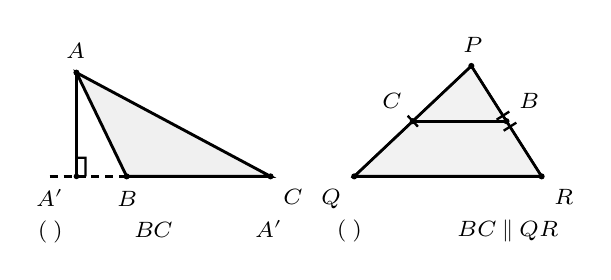
\begin{tikzpicture}[scale=0.85, every node/.style={font=\footnotesize, text=black}]
  % (១) កម្ពស់ក្នុងត្រីកោណមុំទាល (ត្រូវបន្លាយបន្ទាត់ជ្រុងឈម)
  \begin{scope}[shift={(0,0)}]
    \coordinate (B) at (-0.65,0);
    \coordinate (C) at (1.50,0);
    \coordinate (A) at (-1.40,1.55);
    \coordinate (Hp) at (-1.40,0);
    \fill[gray!12] (A) -- (B) -- (C) -- cycle;
    \draw[black, line width=1.05pt] (A) -- (B) -- (C) -- cycle;
    \draw[black, line width=0.85pt, densely dashed] (-1.80,0) -- (B);
    \draw[black, line width=1.0pt] (A) -- (Hp);
    \rightbox[0.18]{A}{Hp}{B}
    \fill[black] (A) circle (1.3pt) node[above=1.5pt] {$A$};
    \fill[black] (B) circle (1.3pt) node[below=2pt] {$B$};
    \fill[black] (C) circle (1.3pt) node[below right=1pt] {$C$};
    \fill[black] (Hp) circle (1.2pt) node[below left=1pt] {$A'$};
    \node at (-0.15,-0.82) {(១) បន្លាយបាត $BC$ រកជើងកម្ពស់ $A'$};
  \end{scope}
  % (២) បន្ទាត់មធ្យមនៃត្រីកោណ PQR
  \begin{scope}[shift={(4.15,0)}]
    \coordinate (Q) at (-1.40,0);
    \coordinate (R) at (1.40,0);
    \coordinate (P) at (0.35,1.65);
    \coordinate (C) at ($(P)!0.5!(Q)$);
    \coordinate (B) at ($(P)!0.5!(R)$);
    \fill[gray!10] (P) -- (Q) -- (R) -- cycle;
    \draw[black, line width=1.0pt] (P) -- (Q) -- (R) -- cycle;
    \draw[black, line width=1.05pt] (C) -- (B);
    \draw[black, line width=0.8pt, tk1] (P) -- (C) (C) -- (Q);
    \draw[black, line width=0.8pt, tk2] (P) -- (B) (B) -- (R);
    \fill[black] (P) circle (1.3pt) node[above=1.5pt] {$P$};
    \fill[black] (Q) circle (1.3pt) node[below left=1pt] {$Q$};
    \fill[black] (R) circle (1.3pt) node[below right=1pt] {$R$};
    \fill[black] (C) circle (1.3pt) node[above left=1pt] {$C$};
    \fill[black] (B) circle (1.3pt) node[above right=1pt] {$B$};
    \node at (0,-0.82) {(២) បន្ទាត់មធ្យម៖ $BC\parallel QR$};
  \end{scope}
\end{tikzpicture}}

% ២. E1 Engage: ផ្លូវកាត់កែងខ្លីបំផុតពីជំរំភ្នំ A, B, C ទៅផ្លូវជាតិឈម (ករណីមុំទាល)
\newcommand{\figEngageALT}{%
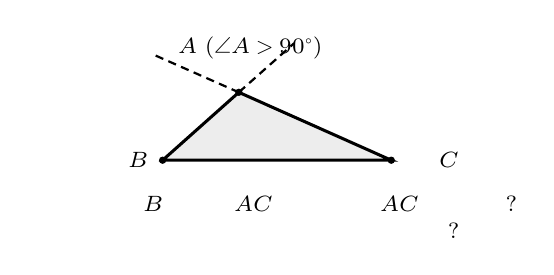
\begin{tikzpicture}[scale=0.88, every node/.style={font=\footnotesize, text=black}]
  \coordinate (B) at (-1.55,-0.30);
  \coordinate (C) at (1.75,-0.30);
  \coordinate (A) at (-0.45,0.68);
  \fill[gray!14] (A) -- (B) -- (C) -- cycle;
  \draw[black, line width=1.1pt] (A) -- (B) -- (C) -- cycle;
  % បន្លាយផ្លូវជ្រុងឈមជាបន្ទាត់ដាច់ៗ
  \draw[black, line width=0.8pt, densely dashed] (-1.65,1.21) -- (A);
  \draw[black, line width=0.8pt, densely dashed] (A) -- (0.35,1.39);
  \fill[black] (A) circle (1.5pt);
  \node at (-0.52,1.32) {ជំរំ $A$ ($\ang{A}>90^\circ$)};
  \fill[black] (B) circle (1.5pt) node[left=2pt] {ជំរំ $B$};
  \fill[black] (C) circle (1.5pt) node[right=2pt] {ជំរំ $C$};
  \node[align=center] at (0.10,-1.12) {តើផ្លូវកាត់កែងពី $B$ ទៅបន្ទាត់ $AC$ កាត់ក្នុងអង្កត់ $AC$ ឬលើបន្លាយក្រៅ?\\តើបន្ទាត់កម្ពស់ទាំងបីអាចប្រសព្វគ្នានៅខាងក្រៅត្រីកោណដែរឬទេ?};
\end{tikzpicture}}

% ២ខ. E2 សកម្មភាពទី១៖ ប្រៀបធៀបទីតាំងអរតូសង់ H លើករណីមុំស្រួច និងត្រីកោណកែង
\newcommand{\figOrthoCasesALT}{%
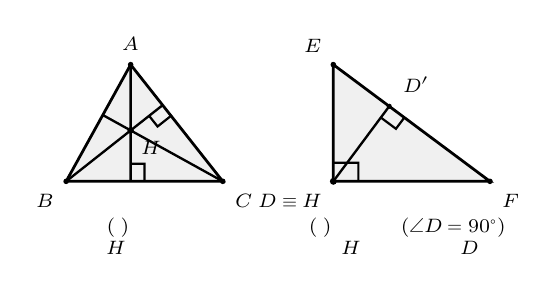
\begin{tikzpicture}[scale=0.78, every node/.style={font=\scriptsize, text=black}]
  % (១) មុំស្រួច៖ H នៅក្នុង
  \begin{scope}[shift={(0,0)}]
    \coordinate (B) at (-1.30,-0.45);
    \coordinate (C) at (1.25,-0.45);
    \coordinate (A) at (-0.25,1.45);
    \coordinate (Ap) at (-0.25,-0.45);
    \coordinate (Bp) at ($(A)!(B)!(C)$);
    \coordinate (Cp) at ($(A)!(C)!(B)$);
    \coordinate (H) at (-0.25,0.38);
    \fill[gray!12] (A) -- (B) -- (C) -- cycle;
    \draw[black, line width=1.0pt] (A) -- (B) -- (C) -- cycle;
    \draw[black, line width=0.85pt] (A) -- (Ap) (B) -- (Bp) (C) -- (Cp);
    \rightbox[0.15]{A}{Ap}{C}
    \rightbox[0.14]{B}{Bp}{C}
    \fill[black] (A) circle (1.3pt) node[above=1.5pt] {$A$};
    \fill[black] (B) circle (1.3pt) node[below left=1pt] {$B$};
    \fill[black] (C) circle (1.3pt) node[below right=1pt] {$C$};
    \fill[black] (H) circle (1.5pt) node[below right=0.5pt] {$H$};
    \node[align=center] at (0,-1.35) {(១) មុំស្រួច៖\\$H$ នៅខាងក្នុង};
  \end{scope}
  % (២) ត្រីកោណកែង៖ H ត្រង់កំពូលមុំកែង D
  \begin{scope}[shift={(4.15,0)}]
    \coordinate (D) at (-1.10,-0.45);
    \coordinate (F) at (1.45,-0.45);
    \coordinate (E) at (-1.10,1.45);
    \coordinate (Dp) at ($(E)!(D)!(F)$);
    \fill[gray!12] (D) -- (E) -- (F) -- cycle;
    \draw[black, line width=1.0pt] (D) -- (E) -- (F) -- cycle;
    \draw[black, line width=0.85pt] (D) -- (Dp);
    \rightbox[0.16]{E}{D}{F}
    \rightbox[0.15]{D}{Dp}{F}
    \fill[black] (D) circle (1.6pt) node[below left=1pt] {$D\equiv H$};
    \fill[black] (F) circle (1.3pt) node[below right=1pt] {$F$};
    \fill[black] (E) circle (1.3pt) node[above left=1pt] {$E$};
    \fill[black] (Dp) circle (1.2pt) node[above right=1.5pt] {$D'$};
    \node[align=center] at (0.15,-1.35) {(២) ត្រីកោណកែង ($\ang{D}=90^\circ$)៖\\$H$ ត្រង់កំពូលមុំកែង $D$};
  \end{scope}
\end{tikzpicture}}

% ៣. E2/E3 ឧទាហរណ៍ ត្រីកោណជំនួយ PQR និង ទ្រឹស្ដីបទអរតូសង់ H (ទំ.២០៨–២០៩)
\newcommand{\figProofALT}{%
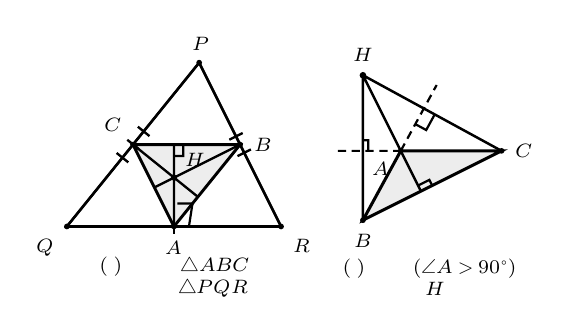
\begin{tikzpicture}[scale=0.80, every node/.style={font=\scriptsize, text=black}]
  % (ក) ឧទាហរណ៍ ទំ.២០៨៖ កម្ពស់នៃ ABC ជាមេដ្យាទ័រនៃ PQR
  \begin{scope}[shift={(0,0)}]
    \coordinate (A) at (0,-0.85);
    \coordinate (B) at (1.05,0.45);
    \coordinate (C) at (-0.65,0.45);
    \coordinate (P) at (0.40,1.75);
    \coordinate (Q) at (-1.70,-0.85);
    \coordinate (R) at (1.70,-0.85);
    \coordinate (Ap) at (0,0.45);
    \coordinate (Bp) at (-0.31,-0.23);
    \coordinate (Cp) at (0.38,-0.38);
    \coordinate (H) at (0,-0.075);

    \draw[black, line width=0.95pt] (P) -- (Q) -- (R) -- cycle;
    \fill[gray!14] (A) -- (B) -- (C) -- cycle;
    \draw[black, line width=1.05pt] (A) -- (B) -- (C) -- cycle;
    \draw[black, line width=0.85pt] (A) -- (Ap) (B) -- (Bp) (C) -- (Cp);
    \rightbox[0.14]{A}{Ap}{B}
    \rightbox[0.14]{P}{A}{R}
    \draw[black, line width=0.75pt, tk1] (Q) -- (A) (A) -- (R);
    \draw[black, line width=0.75pt, tk2] (P) -- (B) (B) -- (R);
    \draw[black, line width=0.75pt, tk3] (P) -- (C) (C) -- (Q);
    \fill[black] (P) circle (1.3pt) node[above=1pt] {$P$};
    \fill[black] (Q) circle (1.3pt) node[below left=1pt] {$Q$};
    \fill[black] (R) circle (1.3pt) node[below right=1pt] {$R$};
    \fill[black] (A) circle (1.3pt) node[below=1.5pt] {$A$};
    \fill[black] (B) circle (1.3pt) node[right=1.5pt] {$B$};
    \fill[black] (C) circle (1.3pt) node[above left=1pt] {$C$};
    \fill[black] (H) circle (1.4pt) node[above right=0.5pt] {$H$};
    \node[align=center] at (0,-1.65) {(ក) កម្ពស់នៃ $\tri{ABC}$\\ជាមេដ្យាទ័រនៃ $\tri{PQR}$};
  \end{scope}

  % (ខ) អរតូសង់ H នៅក្រៅត្រីកោណមុំទាល (ដូចរូបសៀវភៅ ទំ.២០៩)
  \begin{scope}[shift={(4.15,0)}]
    \coordinate (B) at (-1.15,-0.75);
    \coordinate (H) at (-1.15,1.55);
    \coordinate (A) at (-0.55,0.35);
    \coordinate (C) at (1.05,0.35);
    \coordinate (Pb) at (-1.15,0.35);
    \coordinate (Pc) at (-0.183,1.023);
    \coordinate (Pa) at (-0.23,-0.29);

    \fill[gray!14] (A) -- (B) -- (C) -- cycle;
    \draw[black, line width=1.1pt] (A) -- (B) -- (C) -- cycle;
    \draw[black, line width=0.8pt, densely dashed] (-1.55,0.35) -- (A);
    \draw[black, line width=0.8pt, densely dashed] (A) -- ($(B)!1.95!(A)$);
    \draw[black, line width=0.9pt] (B) -- (H) (C) -- (H) (Pa) -- (H);
    \rightbox[0.14]{H}{Pb}{A}
    \rightbox[0.14]{C}{Pc}{B}
    \rightbox[0.14]{A}{Pa}{C}
    \fill[black] (A) circle (1.3pt) node[below left=0.5pt] {$A$};
    \fill[black] (B) circle (1.3pt) node[below=1.5pt] {$B$};
    \fill[black] (C) circle (1.3pt) node[right=1.5pt] {$C$};
    \fill[black] (H) circle (1.5pt) node[above=1.5pt] {$H$};
    \node[align=center] at (-0.05,-1.65) {(ខ) មុំទាល ($\ang{A}>90^\circ$)៖\\អរតូសង់ $H$ នៅក្រៅ};
  \end{scope}
\end{tikzpicture}}

% ៤. E4 លំហាត់គំរូ (ទំ.២០៩–២១០) និង ប្រតិបត្តិ (ទំ.២១០)
\newcommand{\figElaborateALT}{%
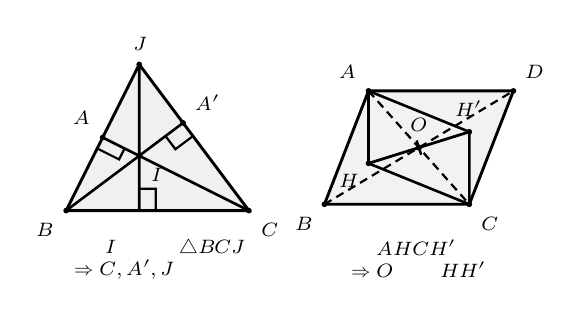
\begin{tikzpicture}[scale=0.80, every node/.style={font=\scriptsize, text=black}]
  % (ក) លំហាត់គំរូ ទំ.២០៩–២១០៖ C, A', J រត់ត្រង់ជួរគ្នា
  \begin{scope}[shift={(0,0)}]
    \coordinate (B) at (-1.45,-0.65);
    \coordinate (C) at (1.45,-0.65);
    \coordinate (J) at (-0.29,1.67);
    \coordinate (K) at (-0.29,-0.65);
    \coordinate (A) at (-0.87,0.51);
    \coordinate (I) at (-0.29,0.22);
    \coordinate (Ap) at (0.406,0.742);

    \fill[gray!12] (B) -- (C) -- (J) -- cycle;
    \draw[black, line width=1.05pt] (B) -- (C) -- (J) -- cycle;
    \draw[black, line width=0.95pt] (C) -- (A) (B) -- (Ap) (J) -- (K);
    \rightbox[0.15]{C}{A}{B}
    \rightbox[0.15]{B}{Ap}{C}
    \rightbox[0.15]{J}{K}{C}
    \fill[black] (B) circle (1.3pt) node[below left=1pt] {$B$};
    \fill[black] (C) circle (1.3pt) node[below right=1pt] {$C$};
    \fill[black] (J) circle (1.3pt) node[above=1.5pt] {$J$};
    \fill[black] (A) circle (1.3pt) node[above left=1pt] {$A$};
    \fill[black] (Ap) circle (1.3pt) node[above right=1pt] {$A'$};
    \fill[black] (I) circle (1.4pt) node[below right=1pt] {$I$};
    \node[align=center] at (0,-1.42) {គំរូ៖ $I$ អរតូសង់នៃ $\tri{BCJ}$\\$\Rightarrow C,A',J$ រត់ត្រង់ជួរ};
  \end{scope}

  % (ខ) ប្រតិបត្តិ ទំ.២១០៖ O កណ្ដាល HH' ក្នុងប្រលេឡូក្រាម ABCD
  \begin{scope}[shift={(4.15,0)}]
    \coordinate (O) at (0,0.35);
    \coordinate (A) at (-0.80,1.25);
    \coordinate (B) at (-1.50,-0.55);
    \coordinate (C) at (0.80,-0.55);
    \coordinate (D) at (1.50,1.25);
    \coordinate (H) at (-0.80,0.10);
    \coordinate (Hp) at (0.80,0.60);

    \fill[gray!10] (A) -- (B) -- (C) -- (D) -- cycle;
    \draw[black, line width=1.05pt] (A) -- (B) -- (C) -- (D) -- cycle;
    \draw[black, line width=0.8pt, densely dashed] (A) -- (C) (B) -- (D);
    \draw[black, line width=0.95pt] (A) -- (H) -- (C) -- (Hp) -- cycle;
    \draw[black, line width=1.0pt, tk1] (H) -- (O) (O) -- (Hp);
    \fill[black] (A) circle (1.3pt) node[above left=1pt] {$A$};
    \fill[black] (B) circle (1.3pt) node[below left=1pt] {$B$};
    \fill[black] (C) circle (1.3pt) node[below right=1pt] {$C$};
    \fill[black] (D) circle (1.3pt) node[above right=1pt] {$D$};
    \fill[black] (O) circle (1.4pt) node[above=2pt] {$O$};
    \fill[black] (H) circle (1.3pt) node[below left=0.5pt] {$H$};
    \fill[black] (Hp) circle (1.3pt) node[above=2pt] {$H'$};
    \node[align=center] at (0,-1.42) {ប្រតិបត្តិ៖ $AHCH'$ ប្រលេឡូក្រាម\\$\Rightarrow O$ កណ្ដាល $HH'$};
  \end{scope}
\end{tikzpicture}}

% ============================================================================
% ចាប់ផ្ដើមឯកសារ (Document Body)
% ============================================================================
\begin{document}
\fontsize{10pt}{15.2pt}\selectfont

% -------------------- ក្បាលកិច្ចតែងការ (Header) --------------------
\begin{center}
  {\muol\fontsize{11pt}{16pt}\selectfont ព្រះរាជាណាចក្រកម្ពុជា}\\[2pt]
  {\muol\fontsize{10pt}{15pt}\selectfont ជាតិ សាសនា ព្រះមហាក្សត្រ}\\[1pt]
  \khmflourish
\end{center}

\vspace{-26pt}
{\muol\fontsize{9.5pt}{12.8pt}\selectfont
មន្ទីរអប់រំ យុវជន និងកីឡា ខេត្តកំពង់ធំ\\
ការិយាល័យអប់រំ យុវជន និងកីឡា ស្រុកកំពង់ស្វាយ\\
អនុវិទ្យាល័យព្រះក្រសាំង}

\vspace{1pt}
\begin{center}
  {\muol\fontsize{10pt}{14.5pt}\selectfont កិច្ចតែងការបង្រៀន}
\end{center}
\vspace{0pt}

% -------------------- ព័ត៌មានទូទៅ (Metadata) --------------------
{\renewcommand{\arraystretch}{0.98}
\hspace*{4.05cm}%
\begin{tabular}{@{}l l l@{}}
  - \hspace{0.35cm} មុខវិជ្ជា & : & គណិតវិទ្យា ថ្នាក់ទី៨ \\
  - \hspace{0.35cm} ចំណងជើងមេរៀន & : & មេរៀនទី១៦ បន្ទាត់និងអង្កត់ពិសេសជួបគ្នានៅក្នុងត្រីកោណ \\
  - \hspace{0.35cm} ចំណងជើងរង & : & ១៦.៣ លក្ខណៈកម្ពស់នៃត្រីកោណ (ទំព័រ ២០៨--២១០) \\
  - \hspace{0.35cm} រយៈពេល & : & ១ ម៉ោងសិក្សា (៥០ នាទី) \\
  - \hspace{0.35cm} បង្រៀនដោយ & : & ហុក ប៊ុនថែន \\
  - \hspace{0.35cm} កាលបរិច្ឆេទ & : & ថ្ងៃ\makebox[18mm]{\dotfill}\ ទី\makebox[8mm]{\dotfill}\ ខែ\makebox[18mm]{\dotfill}\ ឆ្នាំ២០២៦ \\
\end{tabular}

\vspace{2pt}

% -------------------- I. វត្ថុបំណង --------------------
\textbf{I.} {\muol វត្ថុបំណង}\\[1pt]
\hspace*{0.55cm}%
\begin{tabular}{@{}l l L{14.2cm}@{}}
  \wcirc \hspace{0.25cm} វិជ្ជាសម្បទា & : & សិស្សប្រាប់បានត្រឹមត្រូវពីទ្រឹស្ដីបទប្រសព្វកម្ពស់ទាំងបីនៃត្រីកោណ អត្ថន័យនៃអរតូសង់ $H$ ទីតាំងនៃ $H$ តាមប្រភេទត្រីកោណ និងលក្ខណៈសម្គាល់របស់អរតូសង់ ។ \\
  \wcirc \hspace{0.25cm} បំណិនសម្បទា & : & សិស្សប្រើអេគែរនិងបន្ទាត់គូសកម្ពស់ត្រីកោណ (រួមទាំងការបន្លាយបាតចំពោះត្រីកោណមុំទាល) និងប្រើលក្ខណៈអរតូសង់ស្រាយបញ្ជាក់ចំណុចរត់ត្រង់ជួរគ្នា ឬបន្ទាត់កែងគ្នាបានត្រឹមត្រូវ ។ \\
  \wcirc \hspace{0.25cm} ចរិយាសម្បទា & : & សិស្សមានភាពម៉ត់ចត់ក្នុងការប្រើអេគែរវាស់មុំកែង ហ៊ានកែតម្រូវការយល់ច្រឡំលើត្រីកោណមុំទាល និងសហការគ្នាដោះស្រាយបញ្ហាធរណីមាត្រដោយហេតុផល ។ \\
\end{tabular}

\vspace{2pt}

% -------------------- II. សម្ភារៈឧបទេស --------------------
\textbf{II.} {\muol សម្ភារៈឧបទេស}\\[1pt]
\hspace*{0.55cm}$\bullet$ \hspace{0.35cm} សៀវភៅសិក្សាគោលគណិតវិទ្យាថ្នាក់ទី៨ (ទំ.២០៨--២១០, ២១៣--២១៤) សន្លឹកកិច្ចការសិស្ស ស-ខ្មៅ (\en{Worksheet\_ALT} ចំនួន ២ ទំព័រ គ្មាន \en{LCD}) ក្ដារខៀន ដីស បន្ទាត់ក្រិត និងអេគែរ ។

\vspace{2pt}

% -------------------- III. វិធីសាស្រ្តបង្រៀន --------------------
\textbf{III.} {\muol វិធីសាស្រ្តបង្រៀន}\\[1pt]
\hspace*{0.45cm}%
\begin{tabular}{@{}l l L{14.85cm}@{}}
  $\bullet$ \hspace{0.25cm} គោលវិធី & : & សិស្សមជ្ឈមណ្ឌល (សិក្សាតាមរយៈការហ្វឹកហាត់សង់និងបំពេញសន្លឹកកិច្ចការជាគោល គ្មាន \en{LCD}) \\
  $\bullet$ \hspace{0.25cm} យុទ្ធវិធីបង្រៀន & : & ស្ថាបនានិយម គម្រូ \en{5Es} រួមបញ្ចូលការបន្លាយបាតមិនស្តង់ដារ (\en{Non-Prototypical Base-Extension}), សម្រាយបំភ្លឺតាមត្រីកោណជំនួយ $\tri{PQR}$ និងការវិភាគចង្កោមអរតូសង់ ។ \\
\end{tabular}
}

\vspace{2pt}

% -------------------- IV. ដំណើរការបង្រៀន --------------------
\textbf{IV.} {\muol ដំណើរការបង្រៀន}

\vspace{1pt}

\renewcommand{\arraystretch}{1.15}
\begin{longtable}{|L{5.50cm}|L{7.90cm}|L{4.80cm}|}
\hline
\rowcolor{headgray}
\multicolumn{1}{|c|}{\muol សកម្មភាពគ្រូ} &
\multicolumn{1}{c|}{\muol ខ្លឹមសារមេរៀន} &
\multicolumn{1}{c|}{\muol សកម្មភាពសិស្ស} \\
\hline
\endfirsthead

\hline
\rowcolor{headgray}
\multicolumn{1}{|c|}{\muol សកម្មភាពគ្រូ} &
\multicolumn{1}{c|}{\muol ខ្លឹមសារមេរៀន} &
\multicolumn{1}{c|}{\muol សកម្មភាពសិស្ស} \\
\hline
\endhead

\hline
\endfoot

\hline
\endlastfoot

% ==================== ជំហានទី១ (2 min) ====================
\stepheader{ជំហានទី១ (រដ្ឋបាលថ្នាក់)}
$\bullet$ ពិនិត្យវត្តមាន សណ្ដាប់ធ្នាប់ អនាម័យ និងចែកសន្លឹកកិច្ចការ \en{Worksheet\_ALT} ដល់សិស្សគ្រប់គូ \timenote{(2 min)}
&
$\bullet$ រដ្ឋបាលថ្នាក់ និងការត្រៀមបន្ទាត់ក្រិត អេគែរ និងសន្លឹកកិច្ចការសិស្ស
&
$\circ$ ប្រធានថ្នាក់រាយការណ៍វត្តមាន\par\vspace{2pt}
$\circ$ ទទួលសន្លឹកកិច្ចការ និងត្រៀមអេគែរ \\[3pt]
\hline

% ==================== ជំហានទី២ (9 min: ≤3 + 3 + E1 3) ====================
\stepheader{ជំហានទី២ (កិច្ចការផ្ទះ + រំលឹកមេរៀនចាស់ + ទំនាក់ទំនងមេរៀនថ្មី)}
\timenote{(កំណែកិច្ចការផ្ទះ $\le 3\text{ min}$)}\par\vspace{2pt}
$\bullet$ ហៅសិស្ស ១ រូបឡើងបង្ហាញគន្លឹះលំហាត់ទី២ (ទំ.២១៣) និងរំលឹកលទ្ធផលប្រតិបត្តិ (ទំ.២០៨) លើក្ដារខៀន
&
\textbf{កំណែកិច្ចការផ្ទះ (ទំ.២១៣ លំហាត់ទី២)៖}\par\vspace{1.5pt}
ក្នុងប្រលេឡូក្រាម $ABCD$ តាង $O = AC \cap BD$ ($O$ កណ្ដាល $AC$) ។\par\vspace{1.5pt}
ក្នុង $\tri{ABC}$ មេដ្យាន $AJ$ និង $CI$ ប្រសព្វត្រង់ទីប្រជុំទម្ងន់ $G$ ដែលស្ថិតលើមេដ្យានទីបី $BO \subset BD \Rightarrow$ \graybox{$AJ$ និង $CI$ ជួបគ្នាលើ $BD$} ។
&
$\circ$ តំណាងឡើងសរសេរគន្លឹះចម្លើយ\par\vspace{2pt}
$\circ$ ផ្ទៀងផ្ទាត់ចម្លើយក្នុងសៀវភៅសរសេរ \\[3pt]

\timenote{(រំលឹកមេរៀនចាស់ 3 min)}\par\vspace{2pt}
$\bullet$ សួរទី១៖ «តើ \textbf{កម្ពស់} នៃត្រីកោណគូសចេញពីកំពូល $A$ ត្រូវគោរពលក្ខខណ្ឌអ្វី? ចុះបើមុំបាតជាមុំទាល តើជើងកម្ពស់ស្ថិតនៅឯណា?»
&
\textbf{រំលឹកបញ្ញត្តិទាក់ទង៖}\par\vspace{1.5pt}
\ditem \textbf{កម្ពស់នៃត្រីកោណ៖} ជាបន្ទាត់គូសចេញពីកំពូលមួយកាត់កែងនឹង \textbf{បន្ទាត់ជ្រុងឈម} (បើមុំទាល ត្រូវបន្លាយបន្ទាត់ជ្រុងឈមចេញក្រៅ!) ។
&
$\circ$ ឆ្លើយ៖ កាត់តាមកំពូល ហើយកែងនឹងបន្ទាត់ជ្រុងឈម \\[3pt]

$\bullet$ សួរទី២៖ «ក្នុង $\tri{PQR}$ បើ $B$ និង $C$ ជាចំណុចកណ្ដាលនៃ $PR$ និង $PQ$ តើបន្ទាត់ $BC$ និង $QR$ មានទំនាក់ទំនងអ្វី?»
&
\ditem \textbf{បន្ទាត់មធ្យមនៃត្រីកោណ៖}\par\vspace{1.5pt}
បើ $B$ កណ្ដាល $PR$ និង $C$ កណ្ដាល $PQ \Rightarrow BC \parallel QR$ ។\par\vspace{1.5pt}
\ditem \textbf{ប្រសព្វមេដ្យាទ័រ (១៦.២)៖} មេដ្យាទ័រទាំងបីនៃ $\tri{PQR}$ ប្រសព្វគ្នាត្រង់ចំណុចតែមួយ ។
&
$\circ$ ឆ្លើយ៖ $BC \parallel QR$ ហើយមេដ្យាទ័រទាំងបីប្រសព្វគ្នាត្រង់ចំណុចតែមួយ \\[3pt]

& \cfig{\figPrereqALT} & \\[3pt]

\fiveE{E1 - Engage} \timenote{(3 min)}\par\vspace{2pt}
$\bullet$ ណែនាំសិស្សអាន \textbf{បេសកកម្មទី១ (E1)} លើសន្លឹកកិច្ចការទំព័រទី១៖\par\vspace{1.5pt}
\hspace*{0.3em}-- «ជំរំភ្នំទាំងបី $A, B, C$ បង្កើតបានត្រីកោណមុំទាលត្រង់ $A$ ($\ang{A}>90^\circ$)។ បើគេសង់ផ្លូវកាត់កែង ($90^\circ$) ពីជំរំនីមួយៗទៅផ្លូវជ្រុងឈម តើផ្លូវពី $B$ កាត់ក្នុងអង្កត់ $AC$ ឬក្រៅ? ហើយតើបន្ទាត់ផ្លូវទាំងបីអាចជួបគ្នាត្រង់ចំណុច $H$ តែមួយដែរឬទេ?»
&
\textbf{មេរៀនទី១៦៖ បន្ទាត់និងអង្កត់ពិសេសជួបគ្នានៅក្នុងត្រីកោណ}\par\vspace{1.5pt}
\textbf{១៦.៣ លក្ខណៈកម្ពស់នៃត្រីកោណ}\par\vspace{1.5pt}
\ditem \textbf{បញ្ហាបំផុសគំនិត (E1)៖} អន្ទាក់ការគូសកម្ពស់លើត្រីកោណមុំទាល និងការទស្សន៍ទាយពីចំណុចប្រសព្វ $H$ នៃបន្ទាត់កម្ពស់ទាំងបី ។
&
$\circ$ អានបេសកកម្មលើសន្លឹកកិច្ចការ\par\vspace{2pt}
$\circ$ គូសធីកទស្សន៍ទាយជាដៃគូ \\[3pt]

& \cfig{\figEngageALT} & \\[3pt]
\hline

% ==================== ជំហានទី៣ (17 min: E2 11 + E3 6) ====================
\stepheader{ជំហានទី៣ (ខ្លឹមសារមេរៀនថ្មី)}
\fiveE{E2 - Explore} \timenote{(11 min — សកម្មភាពទី១ ហ្វឹកហាត់អេគែរ ៣ ករណី៖ 6 min)}\par\vspace{2pt}
$\bullet$ ឱ្យសិស្សធ្វើការជាដៃគូលើ \textbf{ផ្នែកទី១ (ក) ការសង់កម្ពស់ទាំង ៣ ករណី} ដោយប្រើអេគែរនិងបន្ទាត់ (រួមទាំងត្រីកោណបង្វិលបាត និងត្រីកោណមុំទាល)
&
\textbf{សកម្មភាពរុករកទី១ (សង់កម្ពស់ដោយអេគែរលើ ៣ ករណី)៖}\par\vspace{1.5pt}
$1.$ \textbf{ត្រីកោណមុំស្រួច៖} កម្ពស់ទាំងបីប្រសព្វគ្នាត្រង់ $H$ \textbf{ខាងក្នុង} ត្រីកោណ\par\vspace{1.5pt}
$2.$ \textbf{ត្រីកោណកែង ($\ang{D}=90^\circ$)៖} ជ្រុងកែងទាំងពីរជាកម្ពស់ស្រាប់ $\Rightarrow H \equiv D$ (\textbf{ត្រង់កំពូលមុំកែង})
&
$\circ$ ប្រើអេគែរគូសកម្ពស់លើត្រីកោណមុំស្រួច និងត្រីកោណកែង \\[3pt]

$\bullet$ ណែនាំពិសេសលើករណីទី៣ (មុំទាល)៖ «កុំគូសបញ្ឆិតទៅចំកណ្ដាលជ្រុង! ត្រូវដាក់បន្ទាត់បន្លាយជ្រុង $AB$ និង $AC$ សិន សឹមដាក់អេគែរកែង!»
&
$3.$ \textbf{ត្រីកោណមុំទាល ($\ang{A}>90^\circ$)៖} ក្រោយបន្លាយជ្រុងឈម និងបន្លាយបន្ទាត់កម្ពស់ទាំងបី វាប្រសព្វគ្នាត្រង់ $H$ នៅ \textbf{ខាងក្រៅ} ត្រីកោណ!
&
$\circ$ បន្លាយជ្រុងជាបន្ទាត់ដាច់ៗ ដាក់អេគែរគូសកម្ពស់ និងបន្លាយរកចំណុចប្រសព្វ $H$ នៅខាងក្រៅ \\[3pt]

& \cfig{\figOrthoCasesALT} & \\[3pt]

\timenote{(E2 សកម្មភាពទី២៖ សម្រាយបំភ្លឺតាមត្រីកោណជំនួយ $\tri{PQR}$ — 5 min)}\par\vspace{2pt}
$\bullet$ ដឹកនាំសិស្សបំពេញ \textbf{ផ្នែកទី១ (ខ) ឧទាហរណ៍ (ទំ.២០៨--២០៩)} លើសន្លឹកកិច្ចការ៖ «ក្នុង $\tri{PQR}$ បើ $B, C$ ជាចំណុចកណ្ដាលនៃ $PR, PQ$ តើ $BC$ និង $RQ$ យ៉ាងម៉េចនឹងគ្នា?»
&
\textbf{ឧទាហរណ៍ (ទំ.២០៨--២០៩)៖} $\tri{PQR}$ មាន $A, B, C$ ជាចំណុចកណ្ដាលជ្រុង $RQ, PR, PQ$ ហើយ $AA', BB', CC'$ ជាកម្ពស់នៃ $\tri{ABC}$ ៖\par\vspace{1.5pt}
$\bullet$ ដោយ $B$ កណ្ដាល $PR$ និង $C$ កណ្ដាល $PQ \Rightarrow BC \parallel RQ$ ។
&
$\circ$ បំពេញជំហានទី១៖ $BC \parallel RQ$ \\[3pt]

$\bullet$ សួរបន្ត៖ «បើ $AA'\perp BC$ ហើយ $BC\parallel RQ$ តើ $AA'$ ជាបន្ទាត់អ្វីនៃអង្កត់ $RQ$? ហេតុអ្វីកម្ពស់ទាំងបីនៃ $\tri{ABC}$ ប្រសព្វគ្នាត្រង់ $H$?»
&
$\bullet$ ដោយ $AA'\perp BC$ និង $BC\parallel RQ \Rightarrow AA'\perp RQ$ ត្រង់ចំណុចកណ្ដាល $A \Rightarrow AA'$ ជា \textbf{មេដ្យាទ័រ} នៃ $RQ$ ។\par\vspace{1.5pt}
$\bullet$ ដូចគ្នាដែរ $BB', CC'$ ជាមេដ្យាទ័រនៃ $PR, PQ$ ។ ដោយមេដ្យាទ័រទាំងបីនៃ $\tri{PQR}$ ប្រសព្វគ្នាត្រង់ $H \Rightarrow$ \graybox{កម្ពស់ $AA', BB', CC'$ ប្រសព្វត្រង់ $H$}!
&
$\circ$ បំពេញសន្និដ្ឋាន៖ កម្ពស់នៃ $\tri{ABC}$ គឺជាមេដ្យាទ័រនៃ $\tri{PQR}$ ដូចនេះវាប្រសព្វគ្នាត្រង់ $H$ តែមួយ \\[3pt]

& \cfig{\figProofALT} & \\[3pt]

\fiveE{E3 - Explain} \timenote{(6 min)}\par\vspace{2pt}
$\bullet$ ហៅតំណាងគូសង្ខេប រួចគ្រូសរសេរ \textbf{ទ្រឹស្ដីបទ និងសម្គាល់ (ទំ.២០៩)} លើក្ដារខៀន ឱ្យសិស្សបំពេញ \textbf{ផ្នែកទី២}
&
\textbf{ទ្រឹស្តីបទ (ទំ.២០៩)៖}\par\vspace{1.5pt}
កម្ពស់ទាំងបីនៃត្រីកោណមួយប្រសព្វគ្នាត្រង់ចំណុចតែមួយ ។ ចំណុចប្រសព្វនោះហៅថា \textbf{អរតូសង់} (\en{Orthocenter}) នៃត្រីកោណ (តាងដោយ $H$) ។
&
$\circ$ តំណាងគូបង្ហាញការសន្និដ្ឋាន\par\vspace{2pt}
$\circ$ បំពេញប្រអប់ទ្រឹស្ដីបទលើសន្លឹកកិច្ចការ \\[3pt]

$\bullet$ បញ្ជាក់ \textbf{សម្គាល់សំខាន់ទាំង ២ (ទំ.២០៩)} សម្រាប់ដោះស្រាយលំហាត់ស្រាយបញ្ជាក់
&
\textbf{សម្គាល់ (ទំ.២០៩)៖}\par\vspace{1.5pt}
\ditem ចំណុចមួយនៅលើកម្ពស់ពីរនៃត្រីកោណ ជាអរតូសង់នៃត្រីកោណនោះ វាក៏ឋិតនៅលើកម្ពស់ទីបីដែរ ។\par\vspace{1.5pt}
\ditem ក្នុង \textbf{ត្រីកោណសម័ង្ស} កម្ពស់ក៏ជាមេដ្យាននិងមេដ្យាទ័រ $\Rightarrow O, G, H$ ត្រួតស៊ីគ្នា ។
&
$\circ$ កត់ត្រាសម្គាល់ទាំងពីរចូលក្នុងសន្លឹកកិច្ចការ \\[3pt]

$\bullet$ សួរសង្ខេបប្រៀបធៀបលើក្ដារខៀន៖ «តើទីតាំង $G, O$ និង $H$ ខុសគ្នាយ៉ាងដូចម្ដេចតាមប្រភេទត្រីកោណ?»
&
\textbf{តារាងប្រៀបធៀបចំណុចពិសេស $G, O, H$ លើក្ដារខៀន៖}\par\vspace{2pt}
{\renewcommand{\arraystretch}{1.12}\footnotesize
\begin{tabular}{|L{1.75cm}|L{1.52cm}|L{1.72cm}|L{1.66cm}|}
\hline
\cellcolor{headgray}\textbf{ត្រីកោណ} & \cellcolor{headgray}\textbf{$G$ (មេដ្យាន)} & \cellcolor{headgray}\textbf{$O$ (មេដ្យាទ័រ)} & \cellcolor{headgray}\textbf{$H$ (កម្ពស់)} \\[2pt]
\hline
មុំស្រួច & នៅក្នុង & នៅក្នុង & នៅក្នុង \\
\hline
កែង & នៅក្នុង & កណ្ដាលអ៊ីប៉ូ. & កំពូលមុំកែង \\
\hline
មុំទាល & នៅក្នុង & នៅក្រៅ & នៅក្រៅ \\
\hline
\end{tabular}}
&
$\circ$ ប្រៀបធៀបទីតាំង $G, O, H$ គ្រប់ប្រភេទត្រីកោណ \\[3pt]

$\bullet$ ណែនាំធនាគារហេតុផល \cnum{1}--\cnum{5} សម្រាប់ដោះស្រាយលំហាត់គំរូ និងប្រតិបត្តិ
&
\textbf{ធនាគារហេតុផល (\en{Warrant Bank})៖}\par\vspace{1.5pt}
\cnum{1} និយមន័យកម្ពស់ ($AA'\perp BC$) \;\textbar\; \cnum{2} ប្រសព្វកម្ពស់ ២ $\Rightarrow$ កម្ពស់ទី ៣ កាត់តាម $H$\par\vspace{1.5pt}
\cnum{3} ទីតាំង $H$ (ស្រួច $\to$ ក្នុង, កែង $\to$ កំពូលកែង, ទាល $\to$ ក្រៅ)\par\vspace{1.5pt}
\cnum{4} ឯកតាភាពបន្ទាត់កែងតាមចំណុចមួយ \;\textbar\; \cnum{5} លក្ខណៈអង្កត់ទ្រូងប្រលេឡូក្រាម
&
$\circ$ ផ្ទៀងផ្ទាត់ធនាគារហេតុផល \cnum{1}--\cnum{5} \\[3pt]
\hline

% ==================== ជំហានទី៤ (20 min: E4 10 + E5 10) ====================
\stepheader{ជំហានទី៤ (ពង្រីកចំណេះដឹង និងវាយតម្លៃ)}
\fiveE{E4 - Elaborate} \timenote{(10 min — លំហាត់គំរូ ទំ.២០៩--២១០៖ 5 min)}\par\vspace{2pt}
$\bullet$ ដឹកនាំសិស្សអានប្រធាន \textbf{ផ្នែកទី៣ (ក) លំហាត់គំរូ (ទំ.២០៩--២១០)} លើសន្លឹកកិច្ចការទំព័រទី២ និងកំណត់ត្រីកោណធំ $\tri{BCJ}$
&
\textbf{លំហាត់គំរូ (ទំ.២០៩--២១០)៖} $\tri{ABC}$ និង $\tri{A'BC}$ កែងត្រង់ $A$ និង $A'$ មានអ៊ីប៉ូតេនុស $BC$ រួម ។ $I = AC \cap A'B$ ហើយបន្ទាត់កែងនឹង $BC$ តាម $I$ ជួប $AB$ ត្រង់ $J$ ។ បង្ហាញថា $C, A', J$ រត់ត្រង់ជួរគ្នា ។
&
$\circ$ អានប្រធាន និងសង្កេតត្រីកោណ $\tri{BCJ}$ \\[3pt]

$\bullet$ សួរទី១៖ «ក្នុង $\tri{BCJ}$ តើ $CA$ និង $JI$ ជាបន្ទាត់អ្វី? នាំឱ្យចំណុចប្រសព្វ $I$ ជាចំណុចអ្វីនៃ $\tri{BCJ}$?»
&
-- ក្នុង $\tri{BCJ}$៖ $CA\perp BJ$ (កម្ពស់ពី $C$) និង $JI\perp BC$ (កម្ពស់ពី $J$) កាត់គ្នាត្រង់ $I \Rightarrow I$ ជា \textbf{អរតូសង់} នៃ $\tri{BCJ}$ (\cnum{2}) ។
&
$\circ$ បំពេញជំហានទី១៖ $I$ ជាអរតូសង់នៃ $\tri{BCJ}$ \\[3pt]

$\bullet$ សួរបញ្ចប់៖ «បើ $I$ ជាអរតូសង់នៃ $\tri{BCJ}$ តើបន្ទាត់ $BI$ (គឺបន្ទាត់ $A'B$) កែងនឹងបន្ទាត់ណា? ហេតុអ្វី $C, A', J$ រត់ត្រង់ជួរគ្នា?»
&
-- តាម \cnum{2} បន្ទាត់ $BI$ (គឺ $A'B$) ជាកម្ពស់ទីបី $\Rightarrow A'B \perp CJ$ ។\par\vspace{1.5pt}
-- តែ $A'B \perp CA'$ ត្រង់ $A'$ (សម្មតិកម្ម) ។ តាម \cnum{4} បន្ទាត់ $CA'$ និង $CJ$ ត្រួតស៊ីគ្នា $\Rightarrow \graybox{$C, A', J$ រត់ត្រង់ជួរគ្នា}$!
&
$\circ$ បំពេញសន្និដ្ឋានដោយប្រើហេតុផល \cnum{2} និង \cnum{4} \\[3pt]

\timenote{(E4 ប្រតិបត្តិ៖ ទំ.២១០ — 5 min)}\par\vspace{2pt}
$\bullet$ ដឹកនាំសិស្សបំពេញ \textbf{ផ្នែកទី៣ (ខ) ប្រតិបត្តិ (ទំ.២១០)}៖ «បើ $AH\perp BC$ ហើយ $BC\parallel AD$ តើ $AH$ និង $CH'$ (ដែលកែងនឹង $AD$) យ៉ាងម៉េចនឹងគ្នា?»
&
\textbf{ប្រតិបត្តិ (ទំ.២១០)៖} ប្រលេឡូក្រាម $ABCD$ មាន $O = AC \cap BD$, $H$ អរតូសង់នៃ $\tri{ABC}$ និង $H'$ អរតូសង់នៃ $\tri{ACD}$ ។ បង្ហាញថា $O$ កណ្ដាល $HH'$ ៖\par\vspace{1.5pt}
$1.$ $AH\perp BC$ ហើយ $BC\parallel AD \Rightarrow AH\perp AD$; តែ $CH'\perp AD \Rightarrow AH \parallel CH'$ ។
&
$\circ$ បំពេញជំហានទី១៖ $AH \parallel CH'$ \\[3pt]

$\bullet$ សួរបញ្ចប់៖ «ចុះ $CH$ និង $AH'$? តើចតុកោណ $AHCH'$ ជាអ្វី? ទាញបានអ្វីចំពោះ $O$?»
&
$2.$ ដូចគ្នាដែរ $CH\perp AB \Rightarrow CH\perp CD$ ហើយ $AH'\perp CD \Rightarrow CH \parallel AH'$ ។\par\vspace{1.5pt}
$3.$ ហេតុនេះ $AHCH'$ ជាប្រលេឡូក្រាម (\cnum{5}) ដែលអង្កត់ទ្រូង $AC$ មានចំណុចកណ្ដាល $O \Rightarrow \graybox{$O$ ជាចំណុចកណ្ដាលនៃ $HH'$}$ ។
&
$\circ$ បំពេញជំហានទី២--៣ លើសន្លឹកកិច្ចការ \\[3pt]

& \cfig{\figElaborateALT} & \\[3pt]

\fiveE{E5 - Evaluate} \timenote{(10 min — លំហាត់ទី៤ និងទី៥ ទំ.២១៣៖ 6 min)}\par\vspace{2pt}
$\bullet$ ឱ្យសិស្សធ្វើ \textbf{ផ្នែកទី៤ (ក) ចង្កោមអរតូសង់ (លំហាត់ទី៤ និងទី៥ ទំ.២១៣)} ដោយឯករាជ្យ រួចផ្ទៀងផ្ទាត់ជាដៃគូ
&
\textbf{រង្វាយតម្លៃទី១ — លំហាត់ទី៤ និងទី៥ (ទំ.២១៣)៖}\par\vspace{1.5pt}
$\bullet$ \textbf{លំហាត់ទី៤៖} បើ $H$ ជាអរតូសង់នៃ $\tri{ABC}$ នោះ៖\par\vspace{1pt}
\hspace*{0.4em}-- អរតូសង់នៃ $\tri{ABH}$ គឺកំពូល $\mathbf{C}$ \;\textbar\; អរតូសង់នៃ $\tri{CAH}$ គឺកំពូល $\mathbf{B}$\par\vspace{1pt}
\hspace*{0.4em}-- អរតូសង់នៃ $\tri{BCH}$ គឺកំពូល $\mathbf{A}$ (ចតុភាគីអរតូសង់ $\{A,B,C,H\}$!) ។
&
$\circ$ រកឃើញថាក្នុងចំណោម $\{A,B,C,H\}$ ចំណុចនីមួយៗជាអរតូសង់នៃត្រីកោណបង្កើតដោយ ៣ ចំណុចទៀត! \\[3pt]

$\bullet$ ពិនិត្យចម្លើយលំហាត់ទី៥ (ទំ.២១៣) ជាមួយសិស្សទូទាំងថ្នាក់
&
$\bullet$ \textbf{លំហាត់ទី៥៖} បើអរតូសង់ $H$ នៃ $\tri{ABC}$ ឋិតនៅលើមេដ្យាទ័រនៃអង្កត់ $BC$ នោះមេដ្យាទ័រនោះកាត់តាម $H$ ហើយកែងនឹង $BC \Rightarrow$ វាជាកម្ពស់គូសពី $A$ ផងដែរ $\Rightarrow \tri{ABC}$ ជា \textbf{ត្រីកោណសមបាតកំពូល $A$} ($AB=AC$) ។
&
$\circ$ ផ្ទៀងផ្ទាត់ហេតុផល៖ កម្ពស់និងមេដ្យាទ័រត្រួតស៊ីគ្នា $\Rightarrow$ សមបាតកំពូល $A$ \\[3pt]

\timenote{(E5 បិទបេសកកម្ម E1 និង Exit Check — 4 min)}\par\vspace{2pt}
$\bullet$ សួរបិទបេសកកម្មផ្លូវកាត់កែង E1 ពីដើមម៉ោង
&
\textbf{រង្វាយតម្លៃទី២ — បិទ E1 និង Exit Check៖}\par\vspace{1.5pt}
$\bullet$ \textbf{ចម្លើយ E1៖} ផ្លូវកាត់កែងពី $B$ ត្រូវកាត់លើបន្លាយនៃ $AC$ នៅក្រៅអង្កត់ $AC$ ហើយបន្ទាត់កម្ពស់ទាំងបីជួបគ្នាត្រង់អរតូសង់ $H$ នៅខាងក្រៅត្រីកោណ ។
&
$\circ$ ផ្ទៀងផ្ទាត់ការទស្សន៍ទាយដើមម៉ោង E1 \\[3pt]

$\bullet$ ឱ្យសិស្សគូសវង់ \textbf{Exit Check (ផ្នែកទី៤ ខ)} រួចលើកម្រាមដៃ $1\text{--}4$
&
$\bullet$ \textbf{Exit Check៖} សំណួរទី១ $\to$ \textbf{ក} (កំពូលមុំកែង $A$); សំណួរទី២ $\to$ \textbf{គ} (នៅក្រៅត្រីកោណ); សំណួរទី៣ $\to$ \textbf{ខ} (ត្រីកោណសម័ង្ស) ។
&
$\circ$ គូសវង់ចម្លើយ Exit Check និងលើកម្រាមដៃបង្ហាញ \\[3pt]
\hline

% ==================== ជំហានទី៥ (≤2 min) ====================
\stepheader{ជំហានទី៥ (កិច្ចការផ្ទះ + បណ្ដាំផ្ញើ)}
\timenote{(ចំណាយពេល $\le 2\text{ min}$)}\par\vspace{2pt}
$\bullet$ ដាក់កិច្ចការផ្ទះពីសៀវភៅគោល (ទំ.២១៤)
&
\centerline{\muol កិច្ចការផ្ទះ \enbf{(}ទំ\enbf{.}២១៤ លំហាត់ទី៩\enbf{,} ទី១០ និងទី១១\enbf{)}}\par\vspace{2pt}
$1.$ \textbf{លំហាត់ទី៩ (ទំ.២១៤)៖} ក្នុងប្រលេឡូក្រាម $ABCD$ បន្ទាត់កែងនឹង $BC$ តាម $A$ និងបន្ទាត់កែងនឹង $AC$ តាម $B$ ប្រសព្វត្រង់ $E$ ។ ប្រាប់ប្រភេទនៃ $\tri{CDE}$ ។
&
$\circ$ កត់ត្រាប្រធានលំហាត់ទី៩ \\[3pt]

$\bullet$ ណែនាំគន្លឹះខ្លីសម្រាប់លំហាត់ទី៩ ទី១០ និងទី១១ (ទំ.២១៤)
&
\textit{-- គន្លឹះទី៩៖} $E$ ជាអរតូសង់នៃ $\tri{ABC} \Rightarrow CE\perp AB \parallel CD \Rightarrow \tri{CDE}$ កែងត្រង់ $C$ ។\par\vspace{1.5pt}
$2.$ \textbf{លំហាត់ទី១០ និងទី១១ (ទំ.២១៤)៖} ស្រាយបំភ្លឺថា $AI \perp CJ$ ក្នុងត្រីកោណកែង $\tri{ABC}$ \textit{(គន្លឹះ៖ បន្ទាត់មធ្យម $IJ\parallel AB \perp AC \Rightarrow J$ ជាអរតូសង់នៃ $\tri{ACI}$)} និងសរសេរសម្រាយពេញលេញលំហាត់ទី១១ ($O$ កណ្ដាល $HH'$) ។
&
$\circ$ កត់ត្រាគន្លឹះលំហាត់ទី៩--១១ ចូលសៀវភៅសរសេរ \\[3pt]

$\bullet$ ផ្ដាំផ្ញើសិស្សអានមេរៀនបន្ទាប់ជាមុន និងត្រៀមឧបករណ៍ធរណីមាត្រឱ្យបានគ្រប់គ្នា
&
$3.$ \textbf{អានជាមុន៖} ចំណុច \textbf{១៦.៤ លក្ខណៈកន្លះបន្ទាត់ពុះមុំនៃត្រីកោណ} (ទំ.២១០--២១២)៖\par\vspace{1.5pt}
\hspace*{0.3em}-- រំលឹកលក្ខណៈសម្គាល់ចំណុចមួយស្ថិតលើកន្លះបន្ទាត់ពុះមុំ (ស្មើចម្ងាយពីជ្រុងទាំងពីរនៃមុំ)\par\vspace{1.5pt}
\hspace*{0.3em}-- ត្រៀម \textbf{ដែកឈាន បន្ទាត់ក្រិត រ៉ាប់ព័រទ័រ និងអេគែរ} សម្រាប់សង់រង្វង់ចារឹកក្នុងត្រីកោណនៅម៉ោងក្រោយ ។
&
$\circ$ កត់ត្រាចំណុចអានជាមុន\par\vspace{2pt}
$\circ$ រក្សាសន្លឹកកិច្ចការទុកក្នុងសៀវភៅ និងជម្រាបលាលោកគ្រូ \\[3pt]
\end{longtable}

% -------------------- កាលបរិច្ឆេទ និងហត្ថលេខា --------------------
\vspace{10pt}
\hfill
\begin{minipage}{9.8cm}
  {\centering
    ថ្ងៃ\makebox[16mm]{\dotfill}\ ខែ\makebox[18mm]{\dotfill}\ ឆ្នាំមមី អដ្ឋស័ក ពុទ្ធសករាជ ២៥៧០\\[2pt]
    កំពង់ស្វាយ, ថ្ងៃទី\makebox[10mm]{\dotfill}\ ខែ\makebox[18mm]{\dotfill}\ ឆ្នាំ២០២៦\\[3pt]
    {\muol គ្រូបង្រៀន}\par}
  \vspace{32pt}
  \hfill{\muol ហុក ប៊ុនថែន}\hspace*{1.4cm}
\end{minipage}

\end{document}
